% ============================================================
%  DISCOVERY CURRICULUM — Journey 3, Module 3
%  "Eigenvalues and Eigenvectors"
%  Compile with: pdflatex J3_M3.tex  (run twice for references)
% ============================================================

\documentclass[12pt, a4paper]{article}

\usepackage[a4paper, top=2.5cm, bottom=2.5cm, left=2.8cm, right=2.8cm, headheight=15pt]{geometry}
\usepackage{amsmath, amssymb, amsthm}
\usepackage{xcolor}
\usepackage{mdframed}
\usepackage{enumitem}
\usepackage{tikz}
\usetikzlibrary{arrows.meta, positioning, calc}
\usepackage{pgfplots}
\pgfplotsset{compat=1.18}
\usepackage{booktabs}
\usepackage{fancyhdr}
\usepackage{titlesec}
\usepackage{parskip}
\usepackage{hyperref}
\hypersetup{colorlinks=true, linkcolor=NavyBlue, urlcolor=NavyBlue}

\definecolor{NavyBlue}{HTML}{1A3A5C}
\definecolor{MidBlue}{HTML}{2E6DA4}
\definecolor{Gold}{HTML}{C8922A}
\definecolor{LightBlue}{HTML}{EBF2FA}
\definecolor{LightGold}{HTML}{FDF4E3}
\definecolor{DarkGrey}{HTML}{3A3A3A}
\definecolor{BoxGreen}{HTML}{E8F5E9}
\definecolor{SidebarGrey}{HTML}{F5F5F5}

\titleformat{\section}{\Large\bfseries\color{NavyBlue}}{}{0em}{}[{\color{MidBlue}\vspace{2pt}\rule{\linewidth}{1.5pt}}]
\titleformat{\subsection}{\large\bfseries\color{MidBlue}}{}{0em}{}

\pagestyle{fancy}
\fancyhf{}
\fancyhead[L]{\small\color{DarkGrey}\textit{Discovery Curriculum}}
\fancyhead[R]{\small\color{DarkGrey}\textit{Journey 3 $\cdot$ Module 3}}
\fancyfoot[C]{\small\color{MidBlue}\thepage}
\renewcommand{\headrulewidth}{0.4pt}

\newmdenv[backgroundcolor=NavyBlue!7,linecolor=NavyBlue,linewidth=2pt,leftline=true,rightline=false,topline=false,bottomline=false,innerleftmargin=14pt,innerrightmargin=10pt,innertopmargin=10pt,innerbottommargin=10pt,skipabove=14pt,skipbelow=10pt]{puzzlebox}
\newmdenv[backgroundcolor=LightGold,linecolor=Gold,linewidth=2pt,leftline=true,rightline=false,topline=false,bottomline=false,innerleftmargin=14pt,innerrightmargin=10pt,innertopmargin=10pt,innerbottommargin=10pt,skipabove=14pt,skipbelow=10pt]{discoverybox}
\newmdenv[backgroundcolor=LightBlue,linecolor=MidBlue,linewidth=1.5pt,roundcorner=4pt,innerleftmargin=14pt,innerrightmargin=10pt,innertopmargin=10pt,innerbottommargin=10pt,skipabove=14pt,skipbelow=10pt]{namebox}
\newmdenv[backgroundcolor=BoxGreen,linecolor=DarkGrey!35,linewidth=1pt,roundcorner=4pt,innerleftmargin=14pt,innerrightmargin=10pt,innertopmargin=10pt,innerbottommargin=10pt,skipabove=14pt,skipbelow=10pt]{reflectionbox}
\newmdenv[backgroundcolor=SidebarGrey,linecolor=Gold,linewidth=1.2pt,leftline=true,rightline=false,topline=false,bottomline=false,innerleftmargin=12pt,innerrightmargin=10pt,innertopmargin=7pt,innerbottommargin=7pt,skipabove=10pt,skipbelow=10pt]{thought}

\newcounter{problem}
\newenvironment{problem}[1][]{\refstepcounter{problem}\par\vspace{6pt}\noindent\textbf{\color{MidBlue}Problem \theproblem}\ifx&#1&\else\ \textit{(#1)}\fi\textbf{.}\enskip}{\par\vspace{4pt}}
\newcounter{deepproblem}
\newenvironment{deepproblem}[1][]{\refstepcounter{deepproblem}\par\vspace{6pt}\noindent\textbf{\color{NavyBlue}$\bigstar$\ Deep Problem \thedeepproblem}\ifx&#1&\else\ \textit{(#1)}\fi\textbf{.}\enskip}{\par\vspace{4pt}}

\begin{document}

\thispagestyle{empty}
\begin{center}
{\small\color{MidBlue}\textbf{DISCOVERY CURRICULUM}\quad$\cdot$\quad\textbf{JOURNEY 3: LINEAR STRUCTURE}}
\vspace{0.6cm}

{\color{NavyBlue}\rule{\linewidth}{2pt}}
\vspace{0.5cm}

{\Huge\bfseries\color{NavyBlue}Module 3}\\[0.3cm]
{\LARGE\bfseries\color{MidBlue}Eigenvalues and Eigenvectors}\\[0.4cm]
{\color{Gold}\rule{0.4\linewidth}{1.2pt}}\\[0.4cm]
{\large\itshape\color{DarkGrey}
Every transformation has preferred directions.\\[0.15cm]
Finding them reveals the hidden structure of everything.}

\vspace{1cm}
\begin{tabular}{rl}
\color{DarkGrey}\textbf{Journey}     & Journey 3 --- Linear Structure \\[4pt]
\color{DarkGrey}\textbf{Module}      & 3 of 6 \\[4pt]
\color{DarkGrey}\textbf{Prerequisites} & J3 Modules 1--2 \\[4pt]
\color{DarkGrey}\textbf{You will discover} & Eigenvalues, diagonalisation, spectral theorem, applications \\[4pt]
\color{DarkGrey}\textbf{Format}      & 8 problems $+$ 3 deep problems $\approx$ 14 pages \\
\end{tabular}
\vspace{1cm}

{\color{NavyBlue}\rule{\linewidth}{2pt}}
\end{center}

\vspace{0.5cm}
\noindent\textbf{The central idea.}
Most vectors, when multiplied by a matrix, change direction. But some special vectors are only stretched or compressed --- they point in the same direction before and after. These are eigenvectors, and the stretch factors are eigenvalues. Finding them is not just a computational trick. It reveals the natural axes of a transformation, solves differential equations, governs the long-run behaviour of dynamical systems, and underpins quantum mechanics.

\newpage

\section{Part 1 \texorpdfstring{---}{--} The Puzzle}

\begin{puzzlebox}
\textbf{The Opening Puzzle.}

A rabbit population on an island is tracked each month. Each month: 60\% of rabbits survive to the next month; survivors give birth so that each rabbit alive in month $n$ produces 1.5 new rabbits; separately, 20\% of the juvenile rabbits from the previous month mature.

Let $\mathbf{x}_n = (a_n, b_n)$ where $a_n$ = adult rabbits, $b_n$ = juvenile rabbits. The transition is:
\[
  \begin{pmatrix}a_{n+1}\\b_{n+1}\end{pmatrix}
  = \begin{pmatrix}0.6 & 0.2 \\ 1.5 & 0\end{pmatrix}
  \begin{pmatrix}a_n\\b_n\end{pmatrix}.
\]

\textbf{Question 1.} Starting from $\mathbf{x}_0 = (100, 50)$, compute $\mathbf{x}_1, \mathbf{x}_2, \mathbf{x}_3$ by hand.

\textbf{Question 2.} Compute $\mathbf{x}_{10}$ (use a calculator). What is the ratio $a_{10}/b_{10}$? What is the ratio $a_9/b_9$? Are they close?

\textbf{Question 3.} What do you expect to happen to the population composition in the long run? Does it settle into a fixed ratio of adults to juveniles?

\textbf{Question 4.} Is there an initial distribution $\mathbf{x}_0$ for which the ratio $a_n/b_n$ is \emph{constant} for all $n$? What would that mean?
\end{puzzlebox}

\section{Part 2 \texorpdfstring{---}{--} Exploration}

\subsection{Step 1: Discovering eigenvectors}

\begin{problem}
\label{prob:eigen_discover}
\begin{enumerate}[label=(\alph*), topsep=2pt]
  \item Apply $A = \begin{pmatrix}2&1\\1&2\end{pmatrix}$ to the vectors $(1,1)$, $(1,-1)$, $(1,0)$, $(0,1)$. For which vectors does $A\mathbf{v}$ point in the same direction as $\mathbf{v}$?
  \item For the vectors in (a) where direction is preserved, compute the scaling factor $\lambda$ such that $A\mathbf{v} = \lambda\mathbf{v}$.
  \item Now apply $B = \begin{pmatrix}0&-1\\1&0\end{pmatrix}$ (a $90°$ rotation) to many vectors. Are there any real vectors $\mathbf{v}$ with $B\mathbf{v} = \lambda\mathbf{v}$ for real $\lambda$? What does this mean geometrically?
  \item The equation $A\mathbf{v} = \lambda\mathbf{v}$ rearranges to $(A - \lambda I)\mathbf{v} = \mathbf{0}$. This has a non-trivial solution if and only if $A - \lambda I$ is \emph{not} invertible --- i.e.\ $\det(A - \lambda I) = 0$. Verify this condition for the eigenvalues you found in (b).
\end{enumerate}
\end{problem}

\begin{problem}
\label{prob:char_poly}
The equation $\det(A - \lambda I) = 0$ is the \textbf{characteristic equation} of $A$.
\begin{enumerate}[label=(\alph*), topsep=2pt]
  \item Compute $\det(A - \lambda I)$ for $A = \begin{pmatrix}2&1\\1&2\end{pmatrix}$. This is a polynomial in $\lambda$ --- the \textbf{characteristic polynomial}.
  \item Solve the characteristic equation. The roots are the eigenvalues $\lambda_1, \lambda_2$.
  \item For each eigenvalue, solve $(A - \lambda_i I)\mathbf{v} = \mathbf{0}$ to find the \textbf{eigenvector}(s).
  \item Repeat for the rabbit matrix $A = \begin{pmatrix}0.6&0.2\\1.5&0\end{pmatrix}$. Find both eigenvalues. For the larger one, find the eigenvector. What does it tell you about the long-run ratio $a_n/b_n$?
  \item For $B = \begin{pmatrix}0&-1\\1&0\end{pmatrix}$: compute the characteristic polynomial and its roots. The roots are complex. What does this mean for real eigenvectors?
\end{enumerate}
\end{problem}

\begin{thought}
\textbf{Why the characteristic polynomial?}
The characteristic polynomial $p(\lambda) = \det(A - \lambda I)$ encodes all eigenvalue information. Its roots are the eigenvalues; its degree equals the matrix size; its coefficients encode invariants (trace, determinant, and more). The \textbf{Cayley-Hamilton theorem} --- which you will prove in the deep problems --- states that $p(A) = 0$: every matrix satisfies its own characteristic equation. This is not a tautology; it is a deep structural fact connecting the polynomial of a number to the matrix equation.
\end{thought}

\subsection{Step 2: Diagonalisation}

\begin{problem}
\label{prob:diag}
If an $n\times n$ matrix $A$ has $n$ linearly independent eigenvectors $\mathbf{v}_1, \ldots, \mathbf{v}_n$ with eigenvalues $\lambda_1, \ldots, \lambda_n$, let $P = [\mathbf{v}_1 \mid \cdots \mid \mathbf{v}_n]$ (eigenvectors as columns).
\begin{enumerate}[label=(\alph*), topsep=2pt]
  \item Show that $AP = PD$ where $D = \text{diag}(\lambda_1, \ldots, \lambda_n)$.
  \item Deduce $A = PDP^{-1}$ (diagonalisation). Verify for $A = \begin{pmatrix}2&1\\1&2\end{pmatrix}$.
  \item Compute $A^{10}$ using $A^{10} = PD^{10}P^{-1}$. How does this compare with direct computation?
  \item Use diagonalisation to find a closed form for $A^n\mathbf{x}_0$ for the rabbit population, where $\mathbf{x}_0 = (100, 50)^T$. Does the dominant eigenvalue determine long-run growth?
  \item \textit{(Connection to ODEs.)} The system $\dot{\mathbf{x}} = A\mathbf{x}$ has solution $\mathbf{x}(t) = e^{tA}\mathbf{x}(0) = Pe^{tD}P^{-1}\mathbf{x}(0)$. Write out what this means explicitly for a $2\times 2$ diagonalisable $A$.
\end{enumerate}
\end{problem}

\begin{center}
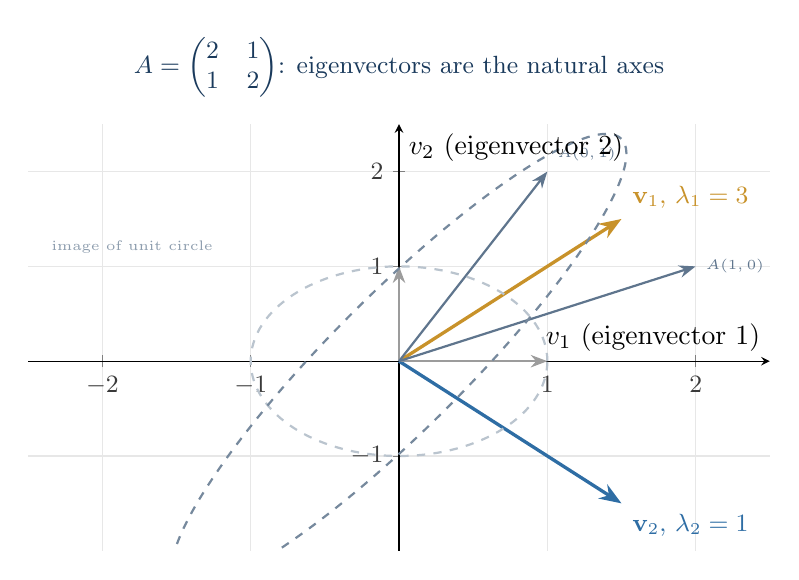
\begin{tikzpicture}
\begin{axis}[
  width=11cm, height=7cm,
  axis lines=center,
  xlabel={$v_1$ (eigenvector 1)}, ylabel={$v_2$ (eigenvector 2)},
  xmin=-2.5, xmax=2.5, ymin=-2, ymax=2.5,
  xtick={-2,-1,1,2}, ytick={-1,1,2},
  tick label style={font=\small, color=DarkGrey},
  grid=major, grid style={DarkGrey!12},
  title={\small\color{NavyBlue}$A = \begin{pmatrix}2&1\\1&2\end{pmatrix}$: eigenvectors are the natural axes},
]
% Eigenvector directions
\draw[-{Stealth[length=8pt]}, Gold, very thick] (axis cs:0,0) -- (axis cs:1.5,1.5) node[above right, font=\small] {$\mathbf{v}_1$, $\lambda_1=3$};
\draw[-{Stealth[length=8pt]}, MidBlue, very thick] (axis cs:0,0) -- (axis cs:1.5,-1.5) node[below right, font=\small] {$\mathbf{v}_2$, $\lambda_2=1$};
% A few generic vectors and their images
\draw[-{Stealth[length=6pt]}, DarkGrey!50, thick] (axis cs:0,0) -- (axis cs:1,0);
\draw[-{Stealth[length=6pt]}, NavyBlue!70, thick] (axis cs:0,0) -- (axis cs:2,1) node[right, font=\tiny] {$A(1,0)$};
\draw[-{Stealth[length=6pt]}, DarkGrey!50, thick] (axis cs:0,0) -- (axis cs:0,1);
\draw[-{Stealth[length=6pt]}, NavyBlue!70, thick] (axis cs:0,0) -- (axis cs:1,2) node[above right, font=\tiny] {$A(0,1)$};
% Ellipse showing stretching
\draw[NavyBlue!30, dashed, thick] (axis cs:0,0) circle [radius=1];
\draw[NavyBlue!60, dashed, thick] (axis cs:0,0) ellipse [x radius=2.12, y radius=0.707, rotate=45];
\node[font=\tiny, color=NavyBlue!50] at (axis cs:-1.8,1.2) {image of unit circle};
\end{axis}
\end{tikzpicture}
\end{center}

\subsection{Step 3: Symmetric matrices and the spectral theorem}

\begin{problem}
\label{prob:spectral}
A matrix $A$ is \textbf{symmetric} if $A = A^T$.
\begin{enumerate}[label=(\alph*), topsep=2pt]
  \item Show that the eigenvalues of a real symmetric matrix are always real. \textit{Hint: suppose $A\mathbf{v} = \lambda\mathbf{v}$; compute $\bar{\mathbf{v}}^T A\mathbf{v}$ two ways, using $A = A^T$.}
  \item Show that eigenvectors of a real symmetric matrix corresponding to distinct eigenvalues are orthogonal.
  \item The \textbf{spectral theorem} states that every real symmetric matrix has an orthonormal basis of eigenvectors (and hence is diagonalisable as $A = Q\Lambda Q^T$ where $Q$ is orthogonal). Verify this for $A = \begin{pmatrix}3&1\\1&3\end{pmatrix}$.
  \item A symmetric matrix is \textbf{positive definite} if all eigenvalues are positive. Show this is equivalent to $\mathbf{x}^T A\mathbf{x} > 0$ for all $\mathbf{x} \neq \mathbf{0}$.
  \item The Hessian matrix from Journey~2 Module~4 is symmetric. The second derivative test says: a critical point is a local minimum if the Hessian is positive definite. Connect this to the eigenvalue condition and explain geometrically why positive-definiteness means a minimum.
\end{enumerate}
\end{problem}

\begin{thought}
\textbf{The spectral theorem is the geometric heart of linear algebra.}
For symmetric matrices, the spectral theorem says: every symmetric transformation has a set of mutually perpendicular axes along which it simply stretches (or compresses). In those axes, the matrix is diagonal --- no rotation, no mixing. This is an extraordinary simplification. The Hessian at a critical point, the covariance matrix of a data set, the inertia tensor of a rigid body, the Hamiltonian of a quantum system --- all are symmetric, and the spectral theorem guarantees they can each be diagonalised in an orthonormal basis. Finding that basis is the act of finding the ``natural frame'' of the system.
\end{thought}

\subsection{Step 4: Applications}

\begin{problem}
\label{prob:pca}
\textbf{Principal Component Analysis (PCA).} A data set has $m$ observations of $n$ features. Stack them in an $m\times n$ matrix $X$ (with columns centred to have mean zero). The \textbf{covariance matrix} is $C = \frac{1}{m}X^T X$.
\begin{enumerate}[label=(\alph*), topsep=2pt]
  \item Show $C$ is symmetric and positive semidefinite (eigenvalues $\geq 0$).
  \item The eigenvectors of $C$ are the \textbf{principal components} --- the directions of maximum variance in the data. The corresponding eigenvalues measure the variance in each direction. Why does the direction of maximum variance correspond to the largest eigenvalue?
  \item For the data points $(1,2), (2,4), (3,5), (4,4), (5,6)$ (centred): compute $C$ and find its eigenvectors. Which direction captures most of the variance?
  \item PCA reduces dimension: project data onto the top $k$ eigenvectors (keep the $k$ largest eigenvalues). What fraction of total variance is retained?
  \item PCA is equivalent to finding the best low-rank approximation of a matrix. This is the \textbf{singular value decomposition} (SVD) --- the subject of Module~4. Write one sentence connecting eigenvectors of $C = X^TX$ to the SVD of $X$.
\end{enumerate}
\end{problem}

\begin{problem}
\label{prob:pagerank}
\textbf{Google PageRank.} The web is a directed graph. Define the $n\times n$ transition matrix $A$ where $A_{ij} = 1/d_j$ if there is a link from page $j$ to page $i$ ($d_j$ = out-degree of $j$), and 0 otherwise.
\begin{enumerate}[label=(\alph*), topsep=2pt]
  \item The PageRank vector $\mathbf{r}$ satisfies $A\mathbf{r} = \mathbf{r}$, i.e.\ $\mathbf{r}$ is an eigenvector with eigenvalue 1. Show that $\mathbf{r}_i$ measures the probability that a random surfer is on page $i$ in the long run.
  \item The \textbf{Perron-Frobenius theorem} states that a positive matrix has a unique eigenvector with all positive entries corresponding to its largest eigenvalue $\lambda_{\max}$. For transition matrices, $\lambda_{\max} = 1$. Why does PageRank exist and why is it unique?
  \item Compute PageRank for a 4-page web: $1 \to 2,3$; $2 \to 3$; $3 \to 1$; $4 \to 1,2,3$. Set up $A$ and find the dominant eigenvector (power iteration: start from $(1,1,1,1)/4$ and repeatedly apply $A$).
  \item The actual Google algorithm adds a ``teleportation'' term: $A' = 0.85A + 0.15(\mathbf{1}\mathbf{1}^T/n)$. Why is this necessary? What happens to pages with no out-links without it?
\end{enumerate}
\end{problem}

\begin{problem}
\label{prob:markov}
A \textbf{Markov chain} is a sequence of states where the probability of transitioning from state $i$ to state $j$ is $M_{ji}$ (the columns of $M$ sum to 1). The state vector after $n$ steps is $\mathbf{p}_n = M^n\mathbf{p}_0$.
\begin{enumerate}[label=(\alph*), topsep=2pt]
  \item For $M = \begin{pmatrix}0.9&0.3\\0.1&0.7\end{pmatrix}$: find the eigenvalues. What are they?
  \item The stationary distribution $\boldsymbol{\pi}$ satisfies $M\boldsymbol{\pi} = \boldsymbol{\pi}$. Find it.
  \item Show $M^n \to \Pi$ (matrix with $\boldsymbol{\pi}$ as each column) as $n\to\infty$ for any starting $\mathbf{p}_0$. Explain using the eigenvalue decomposition.
  \item The \textbf{spectral gap} $1 - |\lambda_2|$ (where $\lambda_2$ is the second-largest eigenvalue) controls how quickly the chain converges to stationarity. For this matrix, how many steps are needed to get within $1\%$ of stationarity?
  \item Both PageRank and Markov chains involve the dominant eigenvector of a transition matrix. State the common principle they share.
\end{enumerate}
\end{problem}

\section{Part 3 \texorpdfstring{---}{--} Discovery}

\begin{discoverybox}
\textbf{What have we built?}

\textbf{First.} An eigenvector of $A$ is a non-zero vector $\mathbf{v}$ with $A\mathbf{v} = \lambda\mathbf{v}$. Eigenvalues are roots of the characteristic polynomial $\det(A-\lambda I)=0$.

\textbf{Second.} Diagonalisation: if $A$ has $n$ independent eigenvectors, then $A = PDP^{-1}$. This makes powers and exponentials trivial to compute.

\textbf{Third.} The spectral theorem: real symmetric matrices are diagonalisable by an orthogonal matrix. Their eigenvectors are perpendicular; their eigenvalues are real.

\textbf{Fourth.} Applications: population dynamics (dominant eigenvalue $=$ growth rate), PCA (eigenvalues $=$ variance), PageRank and Markov chains (dominant eigenvector $=$ stationary distribution).

\medskip
\textbf{The unifying thread.} Eigenvalues are the natural frequencies of a linear system. Whether you are studying a vibrating string, a quantum particle in a box, or the long-run behaviour of a Markov chain, the eigenvalues tell you what modes of behaviour are possible and the eigenvectors tell you their shape. Finding eigenvalues is, in a profound sense, finding the \emph{spectrum} of a system.
\end{discoverybox}

\section{Part 4 \texorpdfstring{---}{--} Naming the Ideas}

\begin{namebox}
\textbf{Eigenvalues and eigenvectors.}

$A\mathbf{v} = \lambda\mathbf{v}$, $\mathbf{v} \neq \mathbf{0}$. Eigenvalues: roots of $p(\lambda) = \det(A-\lambda I)$.

Eigenspace $E_\lambda = \ker(A - \lambda I)$: a subspace of eigenvectors (plus $\mathbf{0}$).

\textbf{Diagonalisation}: $A = PDP^{-1}$ when $n$ independent eigenvectors exist. \textbf{Spectral theorem}: symmetric $A = Q\Lambda Q^T$ with $Q$ orthogonal and $\Lambda$ real diagonal.

\textbf{Positive definite}: all eigenvalues $>0$; equivalently $\mathbf{x}^T A \mathbf{x} > 0$ for all $\mathbf{x}\neq\mathbf{0}$.
\end{namebox}

\section{Part 5 \texorpdfstring{---}{--} Deep Problems}

\begin{deepproblem}[Cayley-Hamilton and minimal polynomial]
\begin{enumerate}[label=(\alph*)]
  \item The \textbf{Cayley-Hamilton theorem}: every matrix satisfies its own characteristic equation. For $A = \begin{pmatrix}2&1\\1&2\end{pmatrix}$ with $p(\lambda) = \lambda^2 - 4\lambda + 3$, verify $p(A) = A^2 - 4A + 3I = 0$.
  \item Use Cayley-Hamilton to express $A^3$ and $A^4$ for this matrix purely in terms of $A$ and $I$.
  \item The \textbf{minimal polynomial} $m(\lambda)$ is the monic polynomial of lowest degree such that $m(A) = 0$. Show $m(\lambda)$ divides $p(\lambda)$. When are they equal?
  \item For a diagonal matrix $D = \text{diag}(1,1,2)$, find $p(\lambda)$ and $m(\lambda)$. What does a repeated eigenvalue do to the minimal polynomial?
  \item \textit{(Harder.)} Prove Cayley-Hamilton for $2\times 2$ matrices directly by writing $p(\lambda) = \lambda^2 - (\text{tr}\,A)\lambda + \det A$ and computing $p(A)$ in terms of $A^2$, $A$, and $I$.
\end{enumerate}
\end{deepproblem}

\begin{deepproblem}[Jordan normal form]
Not every matrix is diagonalisable. The \textbf{Jordan normal form} is the best diagonal-like form achievable.
\begin{enumerate}[label=(\alph*)]
  \item The matrix $J = \begin{pmatrix}\lambda&1\\0&\lambda\end{pmatrix}$ has only one eigenvalue $\lambda$ but only one independent eigenvector. Show this, and explain why $J$ cannot be diagonalised.
  \item A \textbf{Jordan block} $J_k(\lambda)$ is the $k\times k$ matrix with $\lambda$ on the diagonal, 1 on the superdiagonal, 0 elsewhere. Find the characteristic and minimal polynomials of $J_k(\lambda)$.
  \item Every matrix is similar to a Jordan normal form (a block-diagonal matrix of Jordan blocks). Verify for $A = \begin{pmatrix}3&1&0\\0&3&1\\0&0&3\end{pmatrix}$.
  \item What does the Jordan form tell you about the solution to $\dot{\mathbf{x}} = A\mathbf{x}$ when $A$ is not diagonalisable? How does the presence of a Jordan block of size $k$ change the solution?
  \item \textit{(Philosophical.)} The Jordan form shows that ``almost all'' matrices are diagonalisable (the non-diagonalisable ones form a set of measure zero). Yet Jordan blocks appear constantly in applications (repeated eigenvalues in physical systems). What does this tell us about the role of degeneracy in physics?
\end{enumerate}
\end{deepproblem}

\begin{deepproblem}[Quantum mechanics and Hermitian operators]
In quantum mechanics, the state of a system is a vector in a complex Hilbert space $\mathcal{H}$, and observables (measurable quantities) are represented by \textbf{Hermitian operators} $H = H^\dagger$ (self-adjoint, the complex analogue of symmetric).
\begin{enumerate}[label=(\alph*)]
  \item Prove that the eigenvalues of a Hermitian operator are real. (Repeat the proof of the spectral theorem for symmetric matrices, using complex inner products.)
  \item The \textbf{spectral theorem for Hermitian operators}: a Hermitian operator on a finite-dimensional complex Hilbert space has an orthonormal basis of eigenvectors, all with real eigenvalues. State what this means physically: the possible measurement outcomes for an observable are its eigenvalues, and measurement collapses the state to an eigenvector.
  \item The commutator $[H_1, H_2] = H_1 H_2 - H_2 H_1$ of two Hermitian operators is anti-Hermitian. The \textbf{generalised uncertainty principle} says $\Delta H_1 \cdot \Delta H_2 \geq \frac{1}{2}|\langle[H_1,H_2]\rangle|$. For position $\hat{x}$ and momentum $\hat{p}$ with $[\hat{x},\hat{p}] = i\hbar I$, derive $\Delta x \cdot \Delta p \geq \hbar/2$.
  \item The \textbf{Schr\"odinger equation} $i\hbar\frac{d}{dt}|\psi\rangle = H|\psi\rangle$ has solution $|\psi(t)\rangle = e^{-iHt/\hbar}|\psi(0)\rangle$. If $H$ has eigenstates $|n\rangle$ with eigenvalues $E_n$, write $|\psi(0)\rangle = \sum c_n|n\rangle$ and find $|\psi(t)\rangle$. What oscillates?
  \item \textit{(Research.)} The eigenvalues of the Hamiltonian of a hydrogen atom are $E_n = -13.6/n^2$ eV for $n = 1, 2, 3, \ldots$. These are the energy levels. The differences $E_m - E_n$ correspond to photon frequencies in the emission spectrum. Verify that the Balmer series (visible light) corresponds to transitions to $n=2$ from $n=3,4,5,6$.
\end{enumerate}
\end{deepproblem}

\section{Part 6 \texorpdfstring{---}{--} Reflection}

\begin{reflectionbox}
\textbf{Your reflection task.}

\begin{enumerate}
  \item \textbf{On eigenvectors.} An eigenvector is a direction that a transformation preserves. In your own words: why should any transformation have preferred directions at all? Does every transformation have them? Give an example that does and one that does not (over the reals).

  \item \textbf{On eigenvalues in physics.} The energy levels of a quantum system, the normal modes of a vibrating structure, the natural frequencies of an electrical circuit --- all are eigenvalues of some operator. Does this coincidence feel deep to you, or like an artefact of how we formulate the problems? What would it mean if physical reality genuinely had a discrete spectrum?

  \item \textbf{On PageRank.} Google's ranking algorithm is essentially finding the dominant eigenvector of a transition matrix. This is linear algebra governing what information billions of people see. Write a paragraph: what assumptions in the PageRank model could distort rankings? Could a website manipulate its own eigenvalue?

  \item \textbf{Looking ahead.} Module~4 introduces the SVD, which extends eigendecomposition to non-square matrices. Every matrix --- even rectangular ones --- has a natural set of ``singular values.'' Before you are taught: what do you think the singular values of a matrix measure?
\end{enumerate}
\end{reflectionbox}

\medskip
\noindent\textbf{Looking ahead.}
Module~4 studies the Singular Value Decomposition: the most general decomposition of any matrix, extending the spectral theorem beyond symmetric and square matrices. It is the foundation of modern data science, image compression, and numerical linear algebra.

\vspace{1.4cm}
\begin{center}
{\color{MidBlue}\rule{0.5\linewidth}{0.8pt}}\\[6pt]
{\small\color{DarkGrey}\textit{End of Journey 3, Module 3 --- Eigenvalues and Eigenvectors}}\\[4pt]
{\small\color{DarkGrey}Continue to: \textbf{Module 4 --- Inner Products and the SVD}}\\[6pt]
{\color{MidBlue}\rule{0.5\linewidth}{0.8pt}}
\end{center}

\end{document}